
%(BEGIN_QUESTION)
% Copyright 2010, Tony R. Kuphaldt, released under the Creative Commons Attribution License (v 1.0)
% This means you may do almost anything with this work of mine, so long as you give me proper credit

Three designers are arguing over the best way to install a {\it heat exchanger} to exchange heat between two fluids.  One says the best way is to run the fluids through the exchanger in opposite directions (``contra-flow'').  The second designer claims the best way is to run the fluids through in the same directions.  The third designer says it won't matter either way:

$$\includegraphics[width=15.5cm]{i00610x01.eps}$$

First, identify which of these three designers is correct.

\vskip 10pt

Second, identify whether or not the {\it length} of the heat exchangers is relevant.  In other words, if both heat exchangers were lengthened equally, would this alteration favor one type of flow (contra- versus same-direction) over the other?

\vskip 10pt

Finally, explain the reasoning for both of your answers, being sure to appeal to any relevant principles of thermodynamics.

\underbar{file i00610}
%(END_QUESTION)





%(BEGIN_ANSWER)

Contra-flow is best, regardless of exchanger length.

The reason for this is that contra-flow maximizes the temperature differential between the heating and heated fluids at all points along the exchanger's length.  This is easiest to visualize if the heat exchangers are infinitely long: in the same-flow design the heating and heated fluids will equalize at some temperature between the entering temperatures of the two fluids; in the contra-flow design they will exit at the same temperatures the {\it other} fluid entered at.

\vskip 10pt

3 points for the first answer, and 3 points for the second answer.  4 points for the correct explanation (contingent on getting the first two answers correct).

%(END_ANSWER)





%(BEGIN_NOTES)

{\bf This question is intended for exams only and not worksheets!}.

%(END_NOTES)

